%-------------------------------------------------------------------------------
% yum_subsynth
%-------------------------------------------------------------------------------
%
% \file        yum_subsynth.tex
% \library     Documents
% \author      Chris Ahlstrom
% \date        2015-06-07
% \update      2021-11-28
% \version     $Revision$
% \license     $XPC_GPL_LICENSE$
%
%     Provides the SUBsynth section of yoshimi-user-manual.tex.
%
%-------------------------------------------------------------------------------

\section{SUBsynth}
\label{sec:subsynth}

   The \textsl{Yoshimi} SUBsynth dialog is yet another complex dialog, this time
   for creating a subtractive-synthesis instrument,
   "SUBsynth" or "SUBnote" is a simple engine which makes sounds through
   subtraction of harmonics from white noise.  \cite{zyndoc}

\begin{figure}[H]
   \centering
%  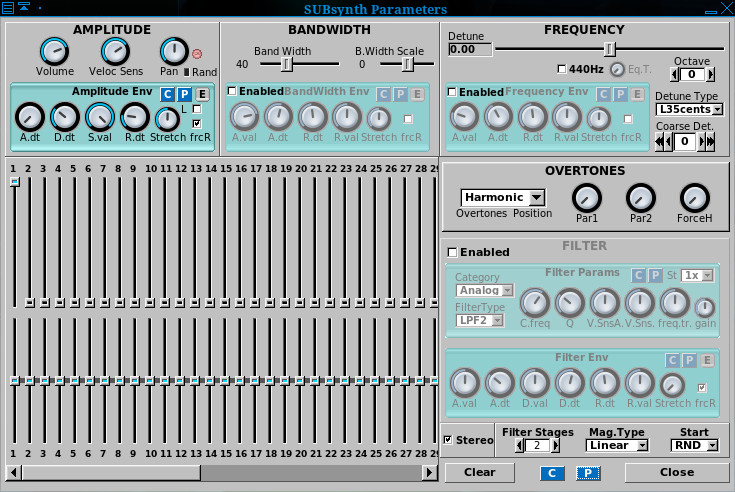
\includegraphics[scale=0.9]{bottom-panel/instrument-edit/SUB/SUBsynth-parameters.jpg}
%  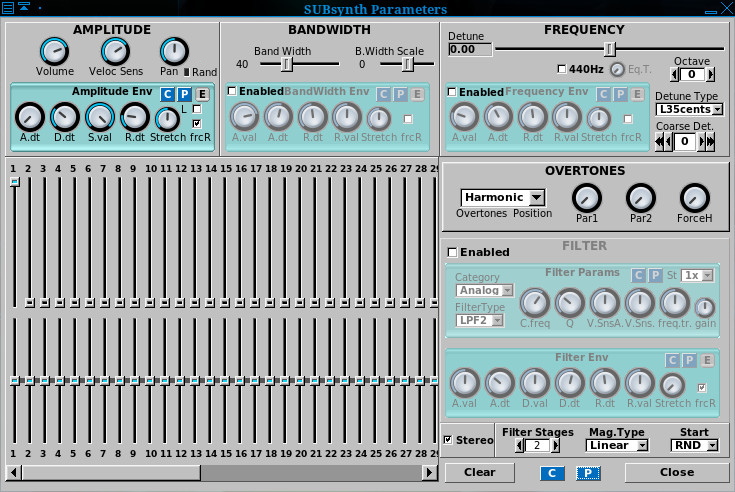
\includegraphics[scale=0.9]{1.4.0/SUBsynth-parameters.png}
%  \includegraphics[scale=0.9]{1.5.0/SubSynth.png}
%  \includegraphics[scale=0.9]{1.7.2/SubSynth.png}
   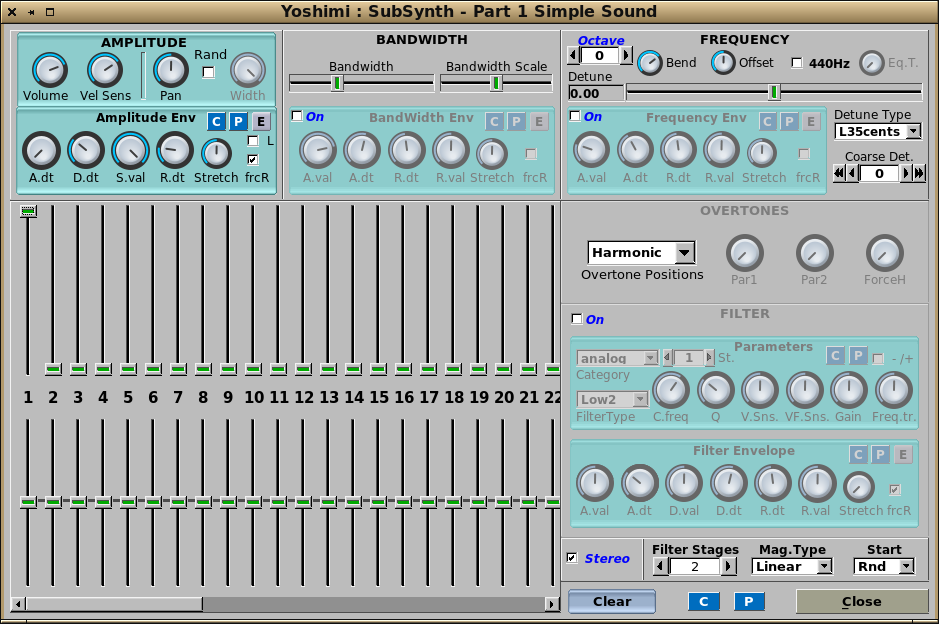
\includegraphics[scale=0.65]{2.1.2/sub.png}
   \caption{SUBsynth Edit Dialog}
   \label{fig:subsynth_edit_dialog}
\end{figure}

   This dialog, though very complex, consists of a number of stock sections
   that are described elsewhere in this manual.
   Some descriptions are repeated here, though.

   \begin{enumber}
      \item \textbf{AMPLITUDE} (section)
      \item \textbf{BANDWIDTH} (section)
      \item \textbf{FREQUENCY} (section)
      \item \textbf{OVERTONES} (section)
      \item \textbf{FILTER} (section)
      \item \textbf{Harmonics} (section)
      \item \textbf{Clear}
      \item \textbf{C}
      \item \textbf{P}
      \item \textbf{Close}
   \end{enumber}

\subsection{SUBsynth / AMPLITUDE}
\label{subsec:subsynth_amplitude}

   \begin{enumber}
      \item \textbf{Volume}
      \item \textbf{Vel Sens}
      \item \textbf{Pan}
      \item \textbf{Rand}
      \item \textbf{Width}

       The controls above are discussed in detail in
       \sectionref{subsec:volume_panning}. However their values for SUBsynth
       are as below.
      \item \textbf{Reset (panning)} (red button)
      \item \textbf{Amplitude Env} (stock sub-panel)
   \end{enumber}

   \setcounter{ItemCounter}{0}      % Reset the ItemCounter for this list.

   \itempar{Volume}{subsynth!volume}

   Values: \texttt{-60dB to 19.4dB, 0dB*}

   \itempar{Vel Sens}{subsynth!vel sens}

   Values: \texttt{-48dB to -0.8dB, disabled, -2.59dB*}

   \itempar{Pan}{subsynth!pan}

   Values: \texttt{100\% left to 100\% right, centered*}

   \itempar{Rand}{subsynth!random pan}

   Values: \texttt{off*, on}

   \itempar{Width}{subsynth!random width}

   Values: \texttt{0 to 100\%* }

   \itempar{Amplitude Env}{subsynth!amplitude envelope}
   Amplitude Envelope.
   See \sectionref{subsubsec:amplitude_envelope_subpanel},
   for information on this stock sub-panel.

\subsection{SUBsynth / BANDWIDTH}
\label{subsec:subsynth_bandwidth}

   \begin{enumber}
      \item \textbf{BandWidth}
      \item \textbf{B.Width Scale}
      \item \textbf{Bandwidth Env}
   \end{enumber}

   \setcounter{ItemCounter}{0}      % Reset the ItemCounter for this list.

   \itempar{BandWidth}{subsynth!bandwidth}
   SUBsynth Bandwidth.
   Sets the bandwidth of each harmonic.

   Values: \texttt{1 to 127, 40*}

   \itempar{B.Width Scale}{subsynth!bandwidth scale}
   SUBsynth Bandwidth Scale.
   Sets how the bandwidth of each harmonic is increased according to the
   frequency. The default (0) increases the bandwidth linearly according to
   the frequency.
   This setting is kind of a "frequency stretch" parameter.

   Values: \texttt{-64 to 63, 0*}

   \itempar{Bandwidth Env}{subsynth!bandwidth envelope}
   SUBsynth Bandwidth.

   \begin{enumber}
      \item \textbf{Enabled}
      \item \textbf{A.val}
      \item \textbf{A.dt}
      \item \textbf{R.dt}
      \item \textbf{R.val}
      \item \textbf{Stretch}
      \item \textbf{frcR}
      \item \textbf{C}
      \item \textbf{P}
      \item \textbf{E}
   \end{enumber}

   \setcounter{ItemCounter}{0}      % Reset the ItemCounter for this list.

   \itempar{Enabled}{bandwidth!enable}
   Enable the panel.

   \itempar{A.val}{bandwidth!attack value}
   Attack value.
   We need to figure out what this means.

   Values: \texttt{0 to 127, 64*}

   \itempar{A.dt}{bandwidth!attack time}
   Attack duration. Attack time.

   Values: \texttt{0 to 127, 40*}

   \itempar{R.dt}{bandwidth!release time}
   Release time.

   Values: \texttt{0 to 127, 60*}

   \itempar{R.val}{bandwidth!release value}
   Release Value.
   Actually present only on the Frequency Env sub-panel.

   Values: \texttt{0 to 127, 64*}

   \itempar{Stretch}{bandwidth!stretch}
   Bandwidth Stretch. On lower notes make the bandwidth lower.

   Values: \texttt{0 to 127, 64*}

   \itempar{frcR}{bandwidth!forced release}
   Forced release.
   If this option is turned on, the release will go to the
   final value, even if the sustain level is not reached.

   Also present in this sub-panel are the usual \textbf{C}opy
   and \textbf{P}aste buttons that call up a copy-parameters or
   paste-parameters dialog, as well as a button
   to bring up the editor window.

   Values: \texttt{Off, On*}

\subsection{SUBsynth / FREQUENCY}
\label{subsec:subsynth_frequency}

   \begin{enumber}
      \item \textbf{Detune}
      \item \textbf{FREQUENCY Slider}
      \item \textbf{Bend}
      \item \textbf{Offset}
      \item \textbf{440Hz}
      \item \textbf{Eq.T}
      \item \textbf{Octave}
      \item \textbf{Detune Type}
      \item \textbf{Coarse Det.}
      \item \textbf{Frequency Env}
   \end{enumber}

   \setcounter{ItemCounter}{0}      % Reset the ItemCounter for this list.

   \itempar{Detune}{subsynth!freq detune}
   Frequency Detune Indicator

   \itempar{FREQUENCY Slider}{subsynth!freq slider}
   Frequency Slider.

   Values: \texttt{-35 to 34.99}

   \itempar{Bend}{voice parameters!bend}
   Bend.
   It modifies the pitch bend control.  It is possible to make the pitch
   bend control work in the opposite direction.

   \itempar{Offset}{voice parameters!offset}
   Offset.
   It shifts the overall pitch of the engine (up or down) relative to the rest
   of the engines.

   \itempar{440Hz}{subsynth!freq 440hz}
   Frequency 440Hz.
   Fixes the base frequency to 440Hz.
   One can adjust it with detune settings.

   \itempar{Eq.T}{subsynth!freq eq t}
   Frequency Equalise Time.
   Sets how the frequency varies according to the keyboard.
   Set to the leftmost setting for a fixed frequency.

   \itempar{Octave}{subsynth!freq octave}
   Frequency Octave.
   Octave Shift.

   \itempar{Detune Type}{subsynth!freq detune type}
   Frequency Detune Type.
   Sets the "Detune" and "Coarse Detune" behaviour

   \itempar{Coarse Det}{subsynth!freq detune coarse}
   Frequency Coarse Detune, "C.Detune".

   \itempar{Frequency Env}{subsynth!freq env}
   Frequency Envelope Stock Sub-Panel.

   \begin{enumber}
      \item \textbf{Enable}
      \item \textbf{A.value} or \textbf{A.val}
      \item \textbf{A.dt}
      \item \textbf{R.dt}
      \item \textbf{R.val}
      \item \textbf{Stretch}
      \item \textbf{frcR}
      \item \textbf{C}
      \item \textbf{P}
      \item \textbf{E}
   \end{enumber}

   See \sectionref{fig:amplitude_envelope_editor}, for more details.

\subsection{SUBsynth / OVERTONES}
\label{subsec:subsynth_overtones}
   By default harmonic overtones are exact multiples of the base frequency, but
   this section allows one to shift them in various unharmonic ways to produce
   metalic or noisy variations.
   \begin{enumber}
      \item \textbf{Overtones Position}
      \item \textbf{Par1}
      \item \textbf{Par2}
      \item \textbf{ForceH}
   \end{enumber}

   \setcounter{ItemCounter}{0}      % Reset the ItemCounter for this list.

   \itempar{Overtones Position}{subsynth!overtone position}
   Subsynth Overtones Position.
   Sets the type of overtone variation. For \textsl{Harmonic} there is no control, so the other parameters are inactive. Similarly \textsl{par2} does nothing for \textsl{Shift} so is disabled for that variation.

   Values: \texttt{Harmonic*, ShiftU, ShiftL, PowerU, PowerL, Sine, Power, Shift}

\begin{figure}[H]
   \centering
   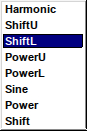
\includegraphics[scale=1.0]{bottom-panel/instrument-edit/SUB/harmonic-type.jpg}
   \caption{Harmonic Type Dropdown}
   \label{fig:harmonic_type_dropdown}
\end{figure}

   \itempar{Par1}{subsynth!overtone par1}
   Subsynth Overtones Par1.
   Spreads the harmonics according to the 'position' type.

   Values: \texttt{0* to 127}

   \itempar{Par2}{subsynth!overtone par1}
   Subsynth Overtones Par2.
   Provides a further variation on the harmonics spread.

   Values: \texttt{0* to 127}

   \itempar{ForceH}{subsynth!overtone forceh}
   Subsynth Overtones ForceH.
   Moves the shifted harmonics by a variable amount towards to the nearest actual multiple of the fundamental.

   Values: \texttt{0* to 127}

\subsection{SUBsynth / FILTER}
\label{subsec:subsynth_filter}

   \begin{enumber}
      \item \textbf{Enabled}
      \item \textbf{Filter Params} (stock sub-panel)
      \item \textbf{Filter Env} (stock sub-panel)
      \item \textbf{Stereo}
      \item \textbf{Filter Stages}
      \item \textbf{Mag. Type}
      \item \textbf{Start}
   \end{enumber}

   \setcounter{ItemCounter}{0}      % Reset the ItemCounter for this list.

   \itempar{Enabled}{subsynth!filter enable}
   SUBsynth Filter Enabled.

   \itempar{Filter Params}{subsynth!filter params}
   Filter Params.  See
   \sectionref{subsubsec:filter_parameters_user_interface},
   which describes this stock sub-panel.

   \itempar{Filter Env}{subsynth!filter env}
   Filter Params.  See
   \sectionref{subsubsec:envelope_settings_for_filter},
   which describes this stock sub-panel.

   \itempar{Stereo}{subsynth!filter stereo}
   SUBsynth Stereo.
   Make the instrument stereo. The CPU usage goes up about 2 times.
   This item isn't really a \textbf{FILTER} item, it is just located in that
   same area.

   \itempar{Filter Stages}{subsynth!filter stages}
   Filter Stages.  Filter Order.
   Sets the number of filter stages applied to white noise. This parameter
   affects the CPU usage.

   Values: \texttt{0, 1, 2*, 3, 4, 5}

   \itempar{Mag. Type}{subsynth!filter mag type}
   Magnitude Type.
   Sets the type of magnitude settings (linear versus dB values)

\begin{figure}[H]
   \centering
   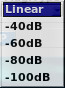
\includegraphics[scale=1.0]{bottom-panel/instrument-edit/SUB/mag-type.jpg}
   \caption{SUBSynth Magnitude Type Dropdown}
   \label{fig:subsynth_magnitude_type_dropdown}
\end{figure}

   Values: \texttt{Linear, -40dB, -60dB, -80dB, -100dB}

   \itempar{Start}{subsynth!filter start type}
   Start Type.
   How to start the filters.

\begin{figure}[H]
   \centering
   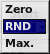
\includegraphics[scale=1.0]{bottom-panel/instrument-edit/SUB/start-type.jpg}
   \caption{SUBsynth Start Type}
   \label{fig:subsynth_start_type}
\end{figure}

   Values: \texttt{Zero, RND, Max.}

\subsection{SUBsynth / Harmonics}
\label{subsec:subsynth_harmonics}

   The harmonics settings controls the harmonic intensities/relative bandwidth.
   Moving the sliders upwards increases the relative bandwidth.  Please note
   that, if one increases the number of harmonics, the CPU usage increases. Right
   click to set the parameters to default values.

   This section consists of 64 sliders to control the amplitude of the narrow
   noise band at a given harmonic, and 64 sliders to control the bandwidth of
   each band.

   The top row of SUBsynth sliders sets the \textsl{relative} amplitude.  This
   use of the word "relative" is an important distinction, as the overall level
   of the output is normalised; all actual levels will be dependent on whichever
   is the highest.

   The bottom row sets the bandwidth of each harmonic. If one has just the
   fundamental, and drops the bandwidth to the minimum, one gets very nearly a
   sinewave.  Set it to maximum and it is very obviously filtered noise.


%-------------------------------------------------------------------------------
% vim: ts=3 sw=3 et ft=tex
%-------------------------------------------------------------------------------
